\specialsection{Приложение}

\begin{figure}[ht]
\begin{flushleft}
\scalebox{0.55}{
   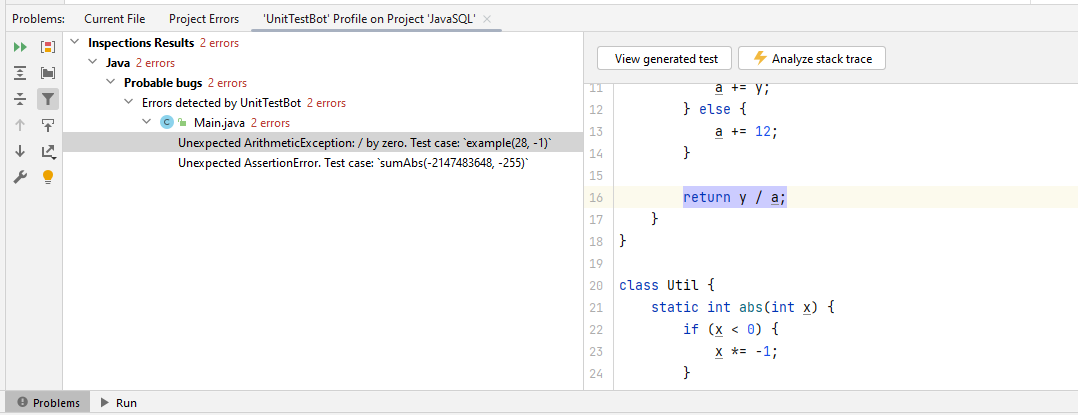
\includegraphics{images/problems-view.png}
}
\caption{
\label{problems-view} Интерфейс просмотра результатов статического анализа.}
\end{flushleft}
\end{figure}

\begin{figure}[ht]
\begin{flushleft}
\scalebox{0.55}{
   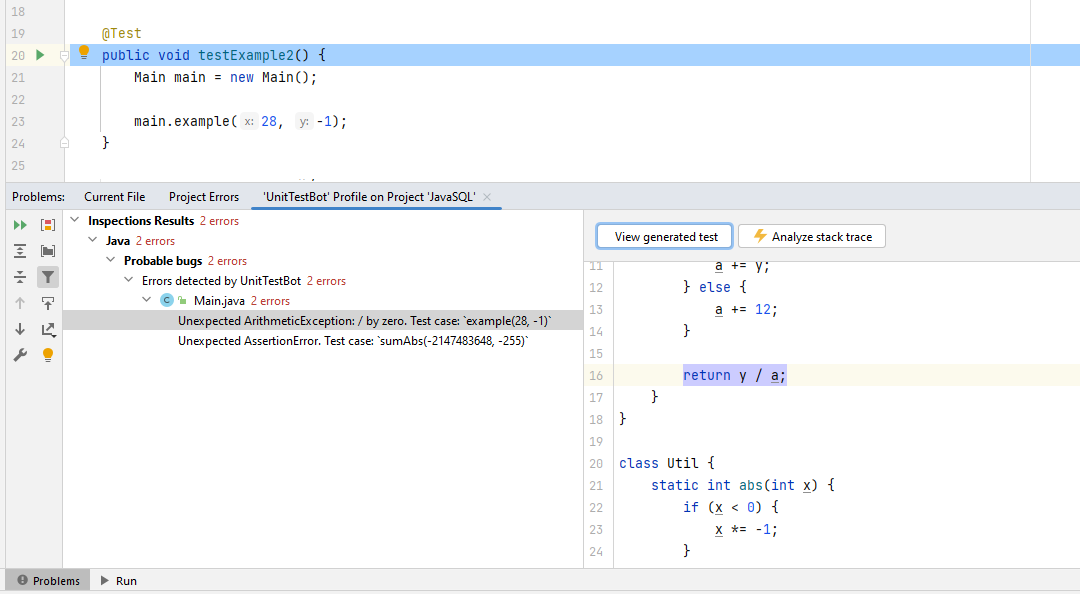
\includegraphics{images/problems-view-test.png}
}
\caption{
\label{problems-view-test} Ссылка на сгенерированный тест.}
\end{flushleft}
\end{figure}

\begin{figure}[ht]
\begin{flushleft}
\scalebox{0.55}{
   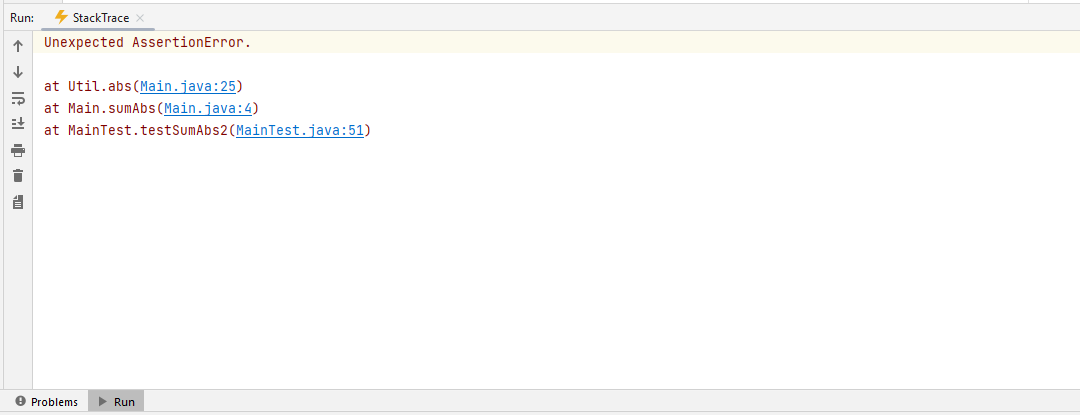
\includegraphics{images/problems-view-stacktrace.png}
}
\caption{
\label{problems-view-stacktrace} Просмотр трассировки стека.}
\end{flushleft}
\end{figure}

\begin{figure}[ht]
\begin{flushleft}
\scalebox{0.55}{
   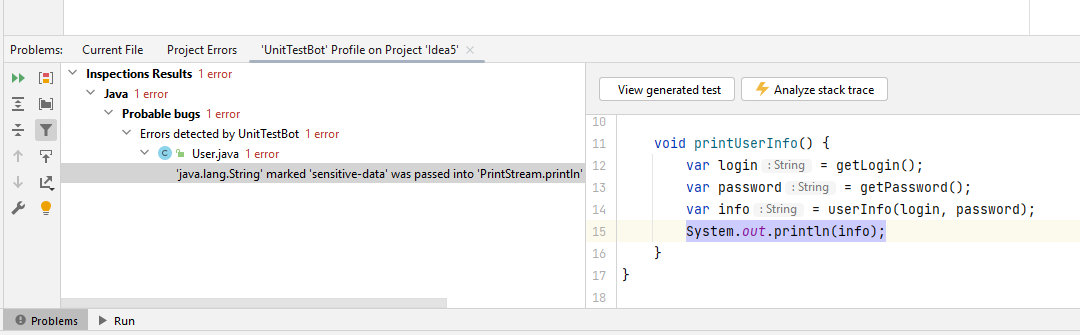
\includegraphics{images/problems-view-taint.png}
}
\caption{
\label{problems-view-taint} Обнаруженная taint-анализом проблема.}
\end{flushleft}
\end{figure}

\definecolor{error-red}{rgb}{1.0, 0.8, 0.8}

\begin{listing}[ht]
\begin{minted}[highlightlines={24},highlightcolor=error-red,linenos,baselinestretch=1,style=abap]{java}
public static int solve(String s) {
    for (int i = 0; i < s.length(); ++i) {
        assume('a' <= s.charAt(i) && s.charAt(i) <= 'z');
    }

    int counter = 0;
    int count = 0;
    while (count < s.length()) {
        counter++;
        char mem1 = s.charAt(count++);
        while (count < s.length() && s.charAt(count) == mem1) {
            count++;
        }
        if (count >= s.length()) {
            break;
        }
        char mem2 = s.charAt(count++);
        while (
            count < s.length() && (s.charAt(count) == mem1 || 
            s.charAt(count) == mem2)
        ) {
            count++;
        }
        char mem3 = s.charAt(count++);
        while (
            count < s.length() && (s.charAt(count) == mem1 || 
            s.charAt(count) == mem2 || s.charAt(count) == mem3)
        ) {
            count++;
        }
    }

    return counter;
}
\end{minted}
\caption{Решение задачи Codeforces-805B, в котором допущена ошибка.}
\label{cf-example}
\end{listing}
